\chapter{Teoría de las curvas elípticas}

\section{Introducción y motivación}
Como hemos mencionado anteriormente en el capítulo~\ref{chap:Campos_finitos}, la eficiencia de los esquemas basados en curvas elípticas depende directamente de la velocidad de los algoritmos de aritmética de curva, que a su vez recaen en las operaciones sobre el campo (suma, multiplicación, inversión)...

La figura~\ref{fig:ECDSA_esquema} muestra las bases necesarias para entender e implementar un protocolo como el algoritmo de firma digital de curva elíptica (ECDSA). La aritmética de curvas no solo se construye sobre las operaciones en el campo subyacente, sino que en algunos casos también requiere aritmética de grandes enteros y operaciones modulares. ECDSA emplea una función hash y ciertas operaciones modulares, pero los pasos más costosos desde el punto de vista computacional son las propias operaciones en la curva.
\begin{figure}[H]
    \centering
    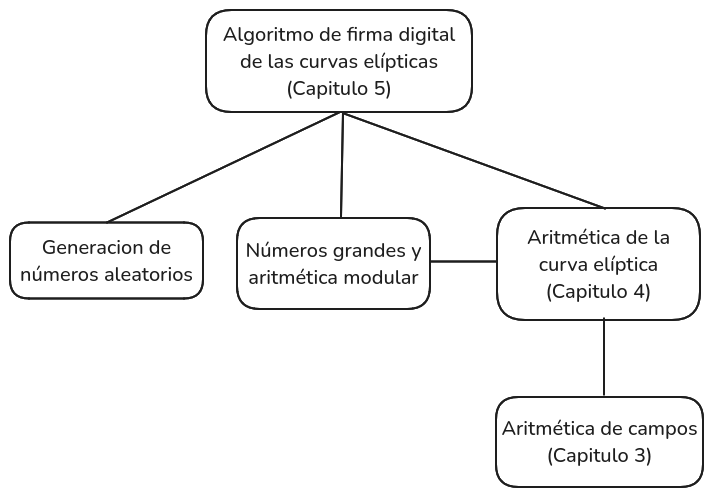
\includegraphics[width=0.8\textwidth]{imagenes/ECDSA_esquema.png}
    \caption{Esquema del Algoritmo de firma digital de las curvas elípticas (ECDSA)}
    \label{fig:ECDSA_esquema}
\end{figure}
%need to update this
La sección~\ref{sec:historia_curvas_elipticas} ofrece una introducción a las curvas elípticas donde se presentan las operaciones de grupo de suma y duplicado para los puntos de la curva, junto con su estructura fundamental y otras propiedades básicas. La sección~3.2 expone las representaciones en coordenadas proyectivas (y los algoritmos asociados de suma y duplicado), de especial interés cuando la inversión en el campo es más cara que la multiplicación. La sección~3.3 discute estrategias para la multiplicación de puntos.

Los métodos de las secciones~3.4, 3.5 y 3.6 están relacionados en que todos ellos explotan endomorfismos de la curva para reducir el coste del duplicado en la multiplicación de puntos. La sección~3.4 trata las curvas de Koblitz especiales, que permiten sustituir el duplicado de punto sobre \(\mathbb{F}_2\) por operaciones de cuadrado en el campo, mucho más baratas. La sección~3.5 examina una clase más amplia de curvas elípticas que admiten endomorfismos usados eficientemente para disminuir el número de duplicaciones. Las estrategias de la sección~3.6, para curvas sobre campos binarios, reemplazan la mayoría de los duplicados por una operación de “halving” de punto, potencialmente más rápida. La sección~3.7 recoge comparaciones de conteo de operaciones para métodos seleccionados de multiplicación de puntos. Finalmente, la sección~3.8 concluye con notas del capítulo y referencias.


\subsection{Historia}\label{sec:historia_curvas_elipticas}


\section{Definición de una curva elíptica}\label{sec:definicion_curvas_elipticas}

\subsection{Forma de Weierstrass general}\label{sec:weierstrass_curvas_elipticas}
\subsection{Transformaciones y cambios de coordenadas}

\section{Estructura de grupo}
\subsection{Punto en el infinito}
\subsection{Ley de suma de puntos (geometría proyectiva)}
\subsection{Propiedades algebraicas}

\section{Curvas sobre cuerpos finitos}\label{sec:curvas_sobre_cuerpos_finitos}
\subsection{Curvas sobre \texorpdfstring{$\mathbb{F}_p$}{Fp}}\label{sec:curvas_sobre_cuerpos_finitos_primos}
\subsection{Curvas binarias sobre \texorpdfstring{$\mathbb{F}_{2^m}$}{F2m}}\label{sec:curvas_sobre_cuerpos_finitos_binarios}

\section{Coordenadas y representación}\label{sec:coordenadas_curvas_elipticas}
\subsection{Coordenadas afines}
\subsection{Coordenadas proyectivas y Jacobianas}
\subsection{Coordenadas 'mixed' y optimizaciones}

\section{Selección de parámetros}
\subsection{Tamaños de curva y seguridad}
\subsection{Cofactores y subgrupos}
\subsection{Curvas estandarizadas (secp256k1, Curve25519, …)}